\documentclass[10pt,a4paper]{article}
\usepackage[utf8]{inputenc}
\usepackage[italian]{babel}
\usepackage{amsmath}
\usepackage{amsfonts}
\usepackage{amssymb}
\usepackage{graphicx}
\usepackage[left=2cm,right=2cm,top=2cm,bottom=2cm]{geometry}
\usepackage{siunitx}
\usepackage{gensymb}
\newcommand{\rem}[1]{[\emph{#1}]}

\author{Gruppo BN \\ Federico Belliardo, Marco Costa, Lisa Bedini}
\title{Ottica 1}
\begin{document}

\maketitle
\section{Scopo dell'esperienza}
Questa esperienza si divide in due parti differenti: A e B.
La parte A è dedicata al calcolo della lunghezza d'onda del sodio, mentre la parte B sfrutta la luce emessa da tre lampade diverse per calcolare la costante di Rydberg e la risoluzione dello spettroscopio a reticolo.\\

\section{Materiale occorrente}
\begin{itemize}
\item lampada al cadmio;
\item lampada al sodio;
\item lampada al mercurio;
\item lampada a idrogeno;
\item elemento dispersivo A: prisma;
\item elemento dispersivo B: reticolo;
\item supporto con goniometro integrato;
\end{itemize}
Inoltre avremo a disposizione due telescopi, uno di raccolta della luce dotato di fenditura per regolare l'intensità del fascio, e uno di osservazione montato sul supporto mobile dotato di goniometro che ruota rispetto alla posizione dell'elemento dispersivo.\\
\section{Parte A - Descrizione esperimento}
\subparagraph{Lampada al cadmio}

Si è rimosso il prisma, quindi abbiamo iniziato la procedura per la taratura dell'apparato sperimentale. Abbiamo posto la lampada al cadmio e i telescopi in modo da allineare il sistema, successivamente abbiamo regolato l'ampiezza della fenditura al minimo per minimizzare l'incertezza. Non abbiamo eseguito una misura dell'angolo $alpha_0$ al quale viene focalizzato il fascio (come sarà invece eseguito nella prossima parte) poiché risulta essere una costante additiva inessenziale nella nostra analisi dati.\\ 
Abbiamo quindi posizionato l'elemento dispersivo con un angolo di almeno $60 \degree$ rispetto alla direzione del telescopio di raccolta e osservato le righe di emissione del cadmio.\\

Nella seguente tabella sono riportate le righe dei colori osservati.


\begin{table}[!htb]
\centering
\begin{tabular}{|c|c|c|}
\hline 
Colore & $\lambda (nm)$ & $\alpha (\degree)$ \\
\hline
Rosso & $643.8\pm0.1$ & $143 \degree 1' \pm 1'$ \\ 
\hline 
Verde & $508.643 \pm 0.001$ & $141 \degree 45' \pm 1'$ \\ 
\hline 
Azzurro & $480.0 \pm 0.1$ & $141 \degree 19' \pm 1'$ \\ 
\hline 
Viola & $467.8 \pm 0.1$	& $141 \degree 5' \pm 1'$ \\ 
\hline 
\end{tabular} 
\label{cadmio}
\end[table}


Come ultima  cosa abbiamo ruotato lentamente il prisma per trovare l'angolo di minima dispersione per la riga verde\footnote{che ha la lunghezza d'onda più vicina a quella del sodio.}, cioè l'angolo di inversione del moto delle righe dello spettro che si osserva muovendo il prisma.\\
Si è dunque eseguita la calibrazione spettrale, nota le lunghezze d'onda delle principali righe di emissione del cadmio. Abbiamo misurato l'angolo di osservazione di ciascuna riga e eseguito un fit lineare $y=ax+b$ nel grafico $\alpha\, \textit{vs}\, 1/\lambda$ ottenendo come parametri $a = -3250 \pm 40 \frac{\degree}{nm}$ e $ b = 148.1 \pm 0.1 \degree$ e $\chi^2=23/2$. Il $\chi^2$ ottenuto è alto a causa del fatto che la curva di calibrazione lineare il funzione di $\frac{1}{\lambda}$ è solo un'approssimazione, ad un comportamenti molto più complesso del prisma.

\begin{figure}[!htb]
  \centering
  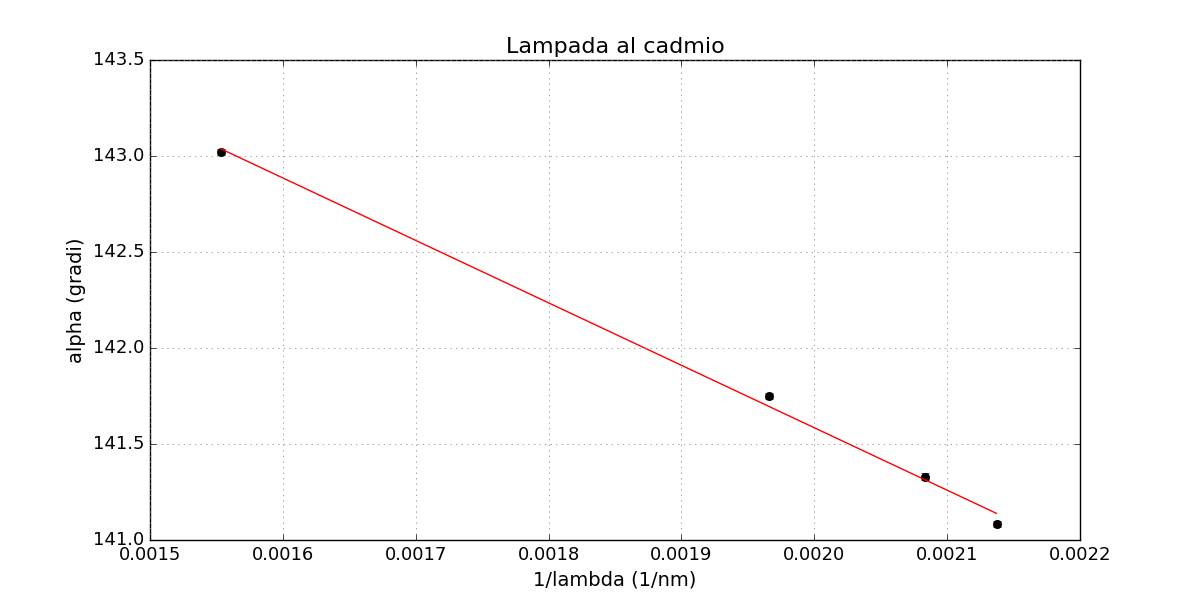
\includegraphics[scale=0.5]{imm.png}
\caption{todo.}
\label{pin}
\end{figure}


\subparagraph{Lampada al sodio}
Si è sostituita la lampada al cadmio con la lampada al sodio precedentemente accesa in modo che si stabilizzasse. Abbiamo individuato la riga\footnote{Un doppietto in realtà ma l'uso del prisma non consente tale risoluzione.} di emissione del sodio e misurata la sua posizione angolare, che risulta $\alpha_{Na}=142 \degree 35'$. Usando le relazioni ricavate precedentemente dal \emph{fit}, si calcola $\lambda_{Na}=590 \pm 10 nm$. Questo valore sarà confrontato con quello ottenuto usando il reticolo, elemento dispersivo con più potere risolutivo del prisma.\\

\section{Parte B - Descrizione esperimento}
\subparagraph{Lampada al mercurio}
Come nella parte precedente, questa prima fase è necessaria per la calibrazione e regolazione dell'apparato sperimentale. Innanzitutto si è posta la lampada al mercurio allineata con la fenditura, quindi abbiamo regolato l'apertura del diaframma in modo da migliorare il rapporto $\frac{segnale}{rumore}$. Abbiamo individuato con il telescopio di osservazione l'ordine zero del reticolo e messo al fuoco gli strumenti, quindi abbiamo controllato che al primo ordine tutte le righe fossero ben visibili.\\
Successivamente abbiamo rimosso la torretta con il reticolo e abbiamo proseguito con la determinazione dell'angolo $\alpha_0$ al quale viene focalizzato il fascio di luce, verificando la coincidenza del centro della riga con la croce sulla lente del telescopio, il risultato ottenuto è $\alpha_0 = 169 \degree 45 '$.\\
Come ultima operazione si è calcolato il passo reticolare. Abbiamo montato la torretta in modo che il telescopio di raccolta e l'elemento dispersivo formassero un angolo di almeno $60 \degree$ e misurato l'angolo di ordine zero della riga verde e l'angolo della stessa riga al primo ordine, i due risultati sono: $\alpha_V^{0} = 227 \degree 53 ' \pm 1'$ e $\alpha_V^{1} = 275 \degree 52' \pm 1'$ \footnote{Tutte le misure angolari riportate nella relazione sono medie delle tre misure eseguite dai tre componenti del gruppo}.

Da semplici considerazioni geometriche si ricavano le seguenti relazioni \footnote{In tutta la relazione abbiamo adottato la convenzione che gli angoli indicati con la lettera $\theta$ sono stati riscalati per il valore di riferimento $\alpha_0$}:

\begin{equation}
\theta_i=\frac{\pi-\theta_0}{2}
\theta_d=\pi-\theta_i-\theta_1
\end{equation}
Quindi è possibile calcolare d sfruttando la relazione del reticolo 
\begin{equation}
d(\sin{\theta_i}-\sin{\theta_d})=m\lambda
\end{equation}

%d =840.2+/-0.5
%N =1190.2+/-0.7
%devo fare propagazione errori massima non statistica

Si ottiene $d = 840.2 \pm 0.5 nm$, che è la spaziatura tra una riga e l'altra del reticolo. Considerando nota la lunghezza d'onda del mercurio $\lambda_{Hg}=546.074\pm0.001\,nm$, quindi si calcola il numero di righe per millimetro $N = 1190 \pm 3$ in accordo con il valore nominale di 1200.


\subparagraph{Lampada a idrogeno}
Si è sostituita la lampada a mercurio con quella a idrogeno, in modo da avere la massima intensità per l'ordine zero senza modificare le distanze focali. Abbiamo quindi misurato la distanza angolare delle righe di emissione per calcolarne le lunghezze d'onda, i risultati sono riportati in tabella \ref{idrogeno}.\\

\begin{table}[!htb]
\centering
\begin{tabular}{|c|c|c|}
\hline 
Viola & $267 \degree 47' \pm 1'$ & $422 \pm 1 nm$ \\ 
\hline 
Azzurro (Int.) & $271 \degree 38' \pm 1'$ & $477 \pm 2 nm$ \\ 
\hline 
Verde (Deb.) & $274 \degree 50' \pm 1'$ & $519 \pm 2 nm$ \\ 
\hline 
Rossa & $283 \degree 15' \pm 1'$ & $649 \pm 1 nm$ \\ 
\hline 
Viola (2° Ord.) & $283\degree 20' \pm 1'$ & _ \\ 
\hline 
\end{tabular} 
\label{idrogeno}
\end{table} 

Attenzione: Il verde forse non è idrogeno

Le lunghezze d'onda sono state calcolate mediante la formula $d(\sin{\theta_i}-\sin{\theta_d})=m\lambda$ e sono riportate nella stessa tabella \ref{idrogeno}.


Lo spettro dell'idrogeno è descritto dall'equazione di Rydberg
\begin{equation}
\frac{1}{\lambda}=R(\frac{1}{n_{1}^2}-\frac{1}{n_{2}^2})
\end{equation}
%n_1=1 Lyman
%n_1=2 Balmer  violetto (n_2=5) azzurro (n_2=4) rosso (n_2=3)
%n_1=3 Paschen

Si è effettuato un fit lineare a un parametro ottenendo un valore per la costante di Rydberg pari a R=  microm^-1 in accordo con il valore atteso pari a $R=10.968\,\textbf{\mum^-1}$. IMMAGINE E DATI FIT.

\subparagraph{Lampada al sodio}
Si è sostituita la lampada a idrogeno con quella al sodio per misurare la lunghezza d'onda del doppietto giallo e confrontare tale dato con quello attenuto nella prima parte dell'esperienza. Al primo ordine abbiamo misurato i seguenti valori angolari $\alpha_{Na,1}= 278 \degree 27' \pm 1 '$ e $\alpha_{Na,2}= 278 \degree 30'$, quindi, sfruttando l'equazione del reticolo si ottiene la lunghezza d'onda $\lambda_{Na,1}= ....$ e $\lambda_{Na,2}= ....$. Tali misure sono compatibili con quelle ottenute precedentemente. La distanza tra le due righe è 0.6nm come atteso. Questo significa anche che la risoluzione dello strumento è almeno 0.6 nm ma dai dati si ottiene come stima sull'errore sistematico 0.4 nm.


\section{Conclusioni}
TUTTO BENE

\end{document}